% !TeX root = main-transferarbeit.tex

%%%%%%%%%%%%%%%%%%%%%%%%%%%%%%%%%%%%%%%%%%%%%%%%%%%%%%%%%%%%%%%%%%%%%%%%%%%%%%%%
%% ABSCHNITT 4: INHALTLICHE BEARBEITUNG
%%
%% Gemäß LIMAK Leitfaden:
%% Hauptteil der Transferarbeit mit Theorie-Praxis-Transfer.
%%
%% Tipps:
%% - Theoretische Grundlagen darstellen (mit Quellenangaben!)
%% - Transfer auf die eigene Praxissituation
%% - Analyse und Reflexion
%% - Entwicklung von Lösungsansätzen
%% - Dieser Abschnitt kann mehrere Unterabschnitte enthalten
%%%%%%%%%%%%%%%%%%%%%%%%%%%%%%%%%%%%%%%%%%%%%%%%%%%%%%%%%%%%%%%%%%%%%%%%%%%%%%%%

\section{Inhaltliche Bearbeitung}
\label{sec:inhaltliche-bearbeitung}

%% TODO: Ersetzen Sie alle Platzhalter [...] mit Ihren eigenen Inhalten.

\subsection{Theoretische Grundlagen}
\label{subsec:theoretische-grundlagen}

%% Stellen Sie hier die relevanten theoretischen Konzepte dar

\subsubsection{[Konzept/Modell 1]}

[Beschreibung des theoretischen Konzepts mit Quellenangaben]

Nach \textcite{Autor2020} bezeichnet [Begriff] ``[Definition]''. Dieses Konzept ist für die vorliegende Fragestellung relevant, weil [Begründung].

Die zentralen Elemente des Konzepts sind:
\begin{itemize}
    \item {[Element 1]}
    \item {[Element 2]}
    \item {[Element 3]}
\end{itemize}

\subsubsection{[Konzept/Modell 2]}

[Beschreibung eines weiteren relevanten Konzepts]

\textcite{AndererAutor2021} betonen die Bedeutung von [Aspekt]. Dies zeigt sich insbesondere in [Beispiel].

%% Beispiel für eine Tabelle:
\begin{table}[htbp]
\centering
\begin{tabular}{@{}lll@{}}
\toprule
\textbf{Aspekt} & \textbf{Beschreibung} & \textbf{Relevanz für Praxis} \\
\midrule
{[Aspekt 1]} & {[Beschreibung]} & {[Relevanz]} \\
{[Aspekt 2]} & {[Beschreibung]} & {[Relevanz]} \\
{[Aspekt 3]} & {[Beschreibung]} & {[Relevanz]} \\
\bottomrule
\end{tabular}
\caption{[Beschreibung der Tabelle]}
\label{tab:konzept-uebersicht}
\end{table}

\subsection{Analyse der Praxissituation}
\label{subsec:analyse-praxis}

%% Analysieren Sie Ihre konkrete Praxissituation im Licht der Theorie

\subsubsection{Ist-Zustand}

[Beschreiben Sie den aktuellen Zustand in Ihrer Praxissituation]

Die Analyse der aktuellen Situation zeigt:
\begin{itemize}
    \item {[Befund 1]}
    \item {[Befund 2]}
    \item {[Befund 3]}
\end{itemize}

\subsubsection{Gap-Analyse}

%% Beispiel für eine Visualisierung mit TikZ
Abbildung~\ref{fig:gap-analyse} zeigt die Lücke zwischen Ist- und Soll-Zustand:

\begin{figure}[htbp]
\centering
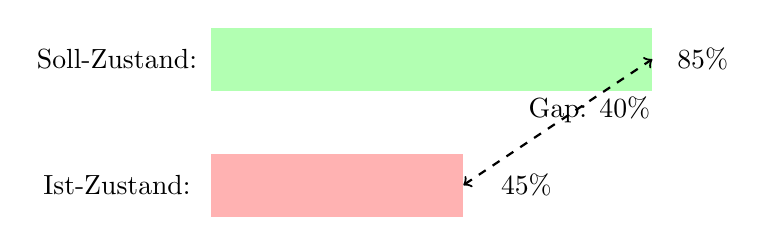
\begin{tikzpicture}[scale=0.8]
  % Ist-Zustand Balken
  \fill[red!30] (0,0) rectangle (4,1);
  \node at (-1.5,0.5) {Ist-Zustand:};
  \node at (5,0.5) {45\%};

  % Soll-Zustand Balken
  \fill[green!30] (0,2) rectangle (7,3);
  \node at (-1.5,2.5) {Soll-Zustand:};
  \node at (7.8,2.5) {85\%};

  % Gap-Markierung
  \draw[<->,thick,dashed] (4,0.5) -- (7,2.5);
  \node at (6,1.7) {Gap: 40\%};
\end{tikzpicture}
\caption{Beispiel: Gap-Analyse Zielerreichung (eigene Darstellung)}
\label{fig:gap-analyse}
\end{figure}

[Vergleichen Sie Ist-Zustand mit dem theoretischen Ideal oder Best Practices]

Verglichen mit den theoretischen Empfehlungen nach \textcite{Autor2020} zeigen sich folgende Lücken:

\begin{enumerate}
    \item \textbf{[Bereich 1]:} [Beschreibung der Lücke]
    \item \textbf{[Bereich 2]:} [Beschreibung der Lücke]
    \item \textbf{[Bereich 3]:} [Beschreibung der Lücke]
\end{enumerate}

\subsection{Lösungsansätze}
\label{subsec:loesungsansaetze}

%% Entwickeln Sie Lösungsansätze basierend auf der Theorie

Auf Basis der theoretischen Erkenntnisse und der Analyse werden folgende Lösungsansätze entwickelt:

\subsubsection{[Lösungsansatz 1]}

[Beschreibung des ersten Lösungsansatzes]

\textbf{Vorteile:}
\begin{itemize}
    \item {[Vorteil 1]}
    \item {[Vorteil 2]}
\end{itemize}

\textbf{Herausforderungen:}
\begin{itemize}
    \item {[Herausforderung 1]}
    \item {[Herausforderung 2]}
\end{itemize}

\subsubsection{[Lösungsansatz 2]}

[Beschreibung des zweiten Lösungsansatzes]

\subsection{Umsetzungskonzept}
\label{subsec:umsetzungskonzept}

%% Beschreiben Sie, wie die Lösungsansätze umgesetzt werden können

\subsubsection{Phasen der Umsetzung}

Die Umsetzung wird in folgende Phasen gegliedert:

\begin{enumerate}
    \item \textbf{Phase 1 -- [Name]:} [Beschreibung]
    \item \textbf{Phase 2 -- [Name]:} [Beschreibung]
    \item \textbf{Phase 3 -- [Name]:} [Beschreibung]
\end{enumerate}

\subsubsection{Erfolgsfaktoren}

Für eine erfolgreiche Umsetzung sind folgende Faktoren kritisch:
\begin{itemize}
    \item {[Erfolgsfaktor 1]}
    \item {[Erfolgsfaktor 2]}
    \item {[Erfolgsfaktor 3]}
\end{itemize}

\subsubsection{Risiken und Gegenmaßnahmen}

\begin{table}[htbp]
\centering
\begin{tabular}{@{}lll@{}}
\toprule
\textbf{Risiko} & \textbf{Eintrittswahrsch.} & \textbf{Gegenmaßnahme} \\
\midrule
{[Risiko 1]} & {[hoch/mittel/niedrig]} & {[Maßnahme]} \\
{[Risiko 2]} & {[hoch/mittel/niedrig]} & {[Maßnahme]} \\
{[Risiko 3]} & {[hoch/mittel/niedrig]} & {[Maßnahme]} \\
\bottomrule
\end{tabular}
\caption{Risiken und Gegenmaßnahmen}
\label{tab:risiken}
\end{table}

